% !TEX root = ../../MathLog.tex

\chapter{Algebra}

\IfLanguageName{english}{\todonote{translate here}}{Die Algebra in ihrer abstrakten Form ist ein Teilgebiet der Mathematik, das sich mit algebraischen Strukturen befasst. Im Gegensatz zur linearen Algebra, welche oft den ersten Kontakt mit algebraischen Strukturen darstellt, wollen wir die abstrakte Algebra ein wenig allgemeiner halten, aber trotzdem mit schönen Beispielen anreichern.

Methoden der Algebra finden Anwendung in fast allen anderen Bereichen der Mathematik und bringen selbst wieder neue Bereiche hervor, wie beispielsweise die Darstellungs- oder Kategorientheorie. Ein sinnvolles Ziel für einen ersten Kurs in Algebra bildet die Aussage, dass die allgemeine Nullstellengleichung eines Polynoms fünften Grades im Gegensatz zu denen kleineren Grades nicht durch Formeln lösbar ist.

\section{Gruppentheorie}

Der erste Teil einer grundlegenden Algebra bildet die Beschäftigung mit Gruppen und ihren Verwandten:

\begin{definition}[Monoid]
  Eine Menge $M$ mit einer Abbildung $\cdot \colon M \times M \rightarrow M$ heißt \emph{Monoid}, falls:
  \begin{enumerate}
    \item $(a \cdot b) \cdot c = a \cdot (b \cdot c)$ für alle $a,b,c \in M$, also $\cdot$ assoziativ.
    \item Es gibt ein $e \in M$, so dass $e \cdot a = a \cdot e = a$ für alle $a \in M$ (ein neutrales Element).
  \end{enumerate}
\end{definition}

Die Abbildung $\cdot$ nennt man auch eine zweistellige Verknüpfung auf $M$. Ist $(M,\cdot)$ nun ein Monoid, so kann man für endlich viele Elemente $a_1, \ldots, a_n \in M$ das \emph{Produkt}:
\[
  \prod_{i=1}^{n} a_i \coloneqq a_1 \cdot \ldots \cdot a_n
\]
definieren, sowie für jedes $a \in M$ und $n \in \NN$ die $n$-te \emph{Potenz} von $a$, mittels:
\[
  a^n \coloneqq \prod_{i=1}^{n} a, \> \mathrm{sowie} \> a^0 = e.
\]

Ein Monoid ist die einfachste algebraische Struktur, die uns zu diesem Zeitpunkt interessieren soll. Lassen wir die Existenz des neutralen Elements fallen, so bildet die dadurch definierte Struktur eine \emph{Halbgruppe}. Lassen wir zusätzlich die Assoziativität weg, so bezeichnen wir $(M,\cdot)$ als \emph{Magma}. Indem wir von einem Monoid nun noch eine weitere Eigenschaft fordern, gelangen wir zum Hauptbegriff dieses Abschnittes:

\begin{definition}[Gruppe]
  Eine Menge $G$ mit einer Abbildung $\cdot \colon G \times G \rightarrow G$ heißt \emph{Gruppe}, falls $(G,\cdot)$ ein Monoid ist, und zusätzlich gilt:
  \begin{enumerate}\setcounter{enumi}{2}
    \item Zu jedem Element $a \in G$ gibt es ein so genanntes \emph{inverses} Element $b \in G$, das heißt: $a \cdot b = b \cdot a = e$.
  \end{enumerate}
  $G$ heißt \emph{kommutativ} oder \emph{abelsch}, falls zusätzlich gilt:
  \begin{enumerate}\setcounter{enumi}{3}
    \item Für alle $a,c \in G$ gilt $a \cdot c = c \cdot a$.
  \end{enumerate}
\end{definition}

Für eine kürzere Schreibweise entscheiden wir uns hier für folgende Notation:

\begin{notation}
  Wir schreiben: $(G,\cdot)$ ist eine Gruppe. Falls die Abbildung $\cdot$ klar ist, schreiben wir nur $G$ für eine Gruppe, und $a \cdot b$ schreiben wir dann nur noch als $ab$.
\end{notation}

Zuerst wollen wir festhalten, dass aus den bisherigen Definitionen bereits zwei fundamentale Charakteristika von Monoiden und Gruppen ableitbar sind:

\begin{proposition}[Eindeutigkeit von neutralen und inversen Elementen]
  Sei $M$ ein Monoid und $G$ eine Gruppe.
  \begin{enumerate}
    \item $M$ (und damit auch jede Gruppe) hat ein eindeutiges neutrales Element.
    \item Jedes Element $a \in G$ hat ein eindeutiges inverses Element.
  \end{enumerate}
\end{proposition}

\begin{proof}
  \begin{enumerate}
    \item Sind $e,e' \in M$ zwei neutrale Elemente, so gilt $e = e \cdot e' = e'$, aufgrund der Definition neutraler Elemente.
    \item Seien $b,b' \in G$ Inverse für $a \in G$. Dann gilt $b' = b' \cdot e = b' \cdot (a \cdot b) = (b' \cdot a) \cdot b = e \cdot b = b$, was ebenfalls aus der Definition folgt.
  \end{enumerate}
\end{proof}

In Zukunft können wir also von \textit{dem} neutralen und inversen Element sprechen. Um einen weiteren Bezug zu uns bekannten Objekten herzustellen, führen wir ein wenig zusätzliche Notation ein.

\begin{notation}[Multiplikative und additive Form]
Sei $(G,\cdot)$ eine Gruppe. Das neutrale Element bezüglich $\cdot$ bezeichnet man oft mit $1$. Das Inverse von $a \in G$ wird dann mit $a^{-1}$ bezeichnet. Dies nennt man die \emph{multiplikative Schreibweise} oder \emph{Form} einer Gruppe.
Die Verknüpfung einer abelschen Gruppe schreibt man oft in \emph{additiver Form}, also $a+b$, $\sum_{i=1}^n a_i$, $n \cdot a = \sum_{i=1}^n a$ bezüglich der Definitionen von vorher. Dann bezeichnet man das neutrale Element mit $0$ und das Inverse von $a \in G$ mit $-a$.
\end{notation}

Wir kennen bereits viele Beispiele für Monoide und Gruppen, die diese Notation nutzen, allerdings werden wir nicht jedes Beispiel beweisen und zusätzlich einige Aussagen als Übungsaufgaben stellen.

\begin{example}[Monoide und Gruppen]
  \leavevmode \vspace{-\baselineskip}
  \begin{enumerate}
    \item $(\ZZ,+)$, $(\QQ,+)$, $(\RR,+)$, $(\CC,+)$ sind abelsche Gruppen.
    \item $(\ZZ,\cdot)$, $(\NN,\cdot)$ sind Monoide, aber keine Gruppen.
    \item $(\QQ,\cdot)$ ist keine Gruppe, denn $0$ hat kein Inverses, allerdings ist $(\QQ^*,\cdot)$ eine Gruppe, wobei $\QQ^* \coloneqq \QQ \setminus \setdef{0}$ ist.
    \item Sei $X$ eine Menge und $(G,\cdot)$ eine Gruppe. Sei $\Abb(X,G)$ die Menge aller Abbildungen von $X$ nach $G$. Definiere $* \colon \Abb(X,G) \times \Abb(X,G) \rightarrow \Abb(X,G)$ durch $(f * g)(x) = f(x) \cdot g(x)$ für jedes $x \in X$.
    Dann bildet $(\Abb(X,G),*)$ eine Gruppe mit dem neutralen Element $e \colon X \rightarrow G$, $e(x) = 1$ für $x \in X$ (hier ist $1 \in G$ das neutrale Element von G). Das Inverse von $f \in \Abb(X,G)$ ist $f^{-1}$ mit $f^{-1}(x) = f(x)^{-1}$.
    \item Sei $\KK$ ein Körper und $\KK^\nn$ die Menge der $\nn$-Matrizen über $\KK$, wobei $n \in \NN$ ist. Dann ist $(\KK^\nn,+)$ eine abelsche Gruppe.
    \item Sei $\GL(n,\KK) \coloneqq \left\{ A \in \KK^\nn \suchthat \det(A) \neq 0 \right\}$ die Menge der invertierbaren $\nn$-Matrizen über $\KK$. Dann ist $(\GL(n,\KK),\cdot)$ eine Gruppe mit der Matrixmultiplikation $\cdot$. Diese Gruppe ist nicht abelsch für $n \geq 2$, dies ist eine Übungsaufgabe.
  \end{enumerate}
\end{example}

Die Abkürzung $\GL$ steht für die \enquote{general linear group}, die allgemeine lineare Gruppe, die diesen Namen trägt, weil $\GL(n,\KK)$ in isomorph ist zur Gruppe der linearen Automorphismen auf $\KK^n$.

\subsection{Untergruppen}

\begin{definition}[Untermonoid, Untergruppe]\label{def:algebra:untergruppe}
  Sei $(G,\cdot)$ ein Monoid. Eine Teilmenge $H \subseteq G$ heißt \emph{Untermonoid}, falls gilt:
  \begin{enumerate}
    \item $e \in H$
    \item Für alle $a, b \in H$ ist auch $ab \in H$.
  \end{enumerate}
  Ist $G$ eine Gruppe, so heißt $H \subseteq G$ \emph{Untergruppe}, falls $H$ ein Untermonoid ist und es gilt:
  \begin{enumerate}\setcounter{enumi}{2}
    \item Für jedes Element $a \in H$ ist auch $a^{-1} \in H$.
  \end{enumerate}
\end{definition}

\begin{notation}[Untergruppe]
  Ist $H \subseteq G$ eine Untergruppe von $G$, so schreibt man $H \leq G$.
\end{notation}

Untergruppen einer Gruppe sind durch Inklusion partiell geordnet. Aus dem Untergruppenverband einer Gruppe lässt sich die Struktur einer Gruppe vollständig ablesen, so können wir große Gruppen allein über ihre Untergruppen verstehen. Zuerst jedoch ein paar Beispiele zu Untergruppen.

\begin{example}
  \leavevmode \vspace{-\baselineskip}
  \begin{enumerate}[label=\alph*)]
    \item In jeder Gruppe $G$ sind $G$ selbst und $\{e\}$ jeweils Untergruppen von $G$. Diese Untergruppen heißen \emph{trivial}.
    \item Sei $m \in \ZZ$ und $m \cdot \ZZ = \left\{m \cdot k \suchthat k \in \ZZ \right\}$. Dann ist $(m\ZZ,+) \leq (\ZZ,+)$, beziehungsweise $m\ZZ \leq \ZZ$ bezüglich $+$.
  \end{enumerate}
\end{example}

\begin{definition}[Erzeugnis]
  Sei $(G,\cdot)$ eine Gruppe.
  \begin{enumerate}
    \item Ist $M \subseteq G$, $M \neq \emptyset$, so ist die Menge
    \[\ip{M} \coloneqq \left\{x_1^{\epsilon_1} \cdot \ldots \cdot x_n^{\epsilon_n} \suchthat n \in \NN, x_i \in M, \epsilon_i \in \{1,-1\}\right\}\] eine Untergruppe von $G$. Diese heißt die von $M$ \emph{erzeugte} Untergruppe von $G$.
    \item $G$ heißt \emph{endlich erzeugt}, wenn es eine endliche Teilmenge $H \subseteq G$ (also $\abs{H} < \infty$) gibt mit $G = \ip{H}$.
    \item $G$ heißt \emph{zyklisch}, falls es ein Element $x \in G$ mit $\ip{\{x\}} = G$ gibt. Dann ist $G = \left\{x^k \suchthat k \in \ZZ \right\}$, denn nach Definition des Erzeugnisses ist \[\ip{\{x\}} = \left\{x \cdot \ldots \cdot x \cdot x^{-1} \cdot \ldots \cdot x^{-1} = x^k \text{ für ein } k \in \ZZ \right\}.\]
  \end{enumerate}
\end{definition}

\begin{notation}[Zyklische Gruppen]
  Oft schreibt man $\ip{x}$ statt $\ip{\{x\}}$.
\end{notation}

\begin{example}[Eine zyklische Gruppe]
  Die ganzen Zahlen $(\ZZ,+)$ sind eine zyklische Gruppe, denn es gilt $\ZZ = \ip{1} = \left\{k \cdot 1 \suchthat k \in \ZZ \right\}$.
\end{example}

\subsection{Homomorphismen und Isomorphismen}

\begin{definition}[Homomorphismus]\label{def:algebra:homomorphismus}
  Seien $(G,\cdot)$ und $(G',\star)$ zwei Monoide mit den neutralen Elementen $e$ und $e'$. Eine Abbildung $\phi \colon G \rightarrow G'$ heißt \emph{Monoidhomomorphismus}, falls die folgenden zwei Eigenschaften gelten:
  \begin{enumerate}
    \item $\phi(e) = e'$ und
    \item $\phi(a \cdot b) = \phi(a) \star \phi(b)$ für alle $a,b \in G$.
  \end{enumerate}
  Sind $G$ und $G'$ sogar Gruppen, so heißt $\phi$ auch \emph{Gruppenhomomorphismus}.
\end{definition}

\begin{lemma}[Homomorphismus-Eigenschaften]
  \leavevmode \vspace{-\baselineskip}
  \begin{enumerate}[label=\alph*)]
    \item Eine Abbildung $\phi \colon G \rightarrow G'$ zwischen Gruppen $(G,\cdot)$ und $(G',\star)$ ist ein Gruppenhomomorphismus genau dann, wenn $\phi(a \cdot b) = \phi(a) \star \phi(b)$ für alle $a,b \in G$ gilt.
    \item Ist $\phi \colon G \rightarrow G'$ ein Gruppenhomomorphismus, so gilt $\phi(a^{-1})=\phi(a)^{-1}$ für alle $a \in G$.
  \end{enumerate}
\end{lemma}

\begin{proof}
  \begin{enumerate}[label=\alph*)]
    \item Die Notwendigkeit von $a)$ ist klar. Wir müssen also nur noch zeigen, dass die erste Eigenschaft aus \reference{Definition}{def:algebra:homomorphismus} gilt. Allerdings ist diese einfach nachzurechnen, es gilt nämlich $\phi(e) = \phi(e \cdot e) = \phi(e) \star \phi(e)$, und da $\phi(e) \in G'$ und $G'$ eine Gruppe ist, existiert ein inverses Element $\phi(e)^{-1}$ für $\phi(e)$.
    Multipliziere die Gleichung mit $\phi(e)^{-1}$, dann erhalten wir $\phi(e) \star \phi(e)^{-1} = \phi(e) \star \phi(e) \star \phi(e)^{-1}$, was nach Auflösen bedeutet, dass $e' = \phi(e)$ gilt.
    \item Es gilt nach der zweiten Eigenschaft von \reference{Definition}{def:algebra:homomorphismus}, dass $\phi(a) \star \phi(a^{-1}) = \phi(a \cdot a^{-1}) = \phi(e) = e'$ ist. Daraus folgt direkt, dass $\phi(a^{-1}) = \phi(a)^{-1}$ sein muss.
  \end{enumerate}
\end{proof}

Gruppenhomomorphismen $\phi \colon G \rightarrow G'$ mit speziellen zusätzlichen Eigenschaften haben noch weitere Bezeichnungen:
\begin{itemize}
  \item $\phi$ ist injektiv, dann ist er ein \emph{Monomorphismus}.
  \item $\phi$ ist surjektiv, dann ist er ein \emph{Epimorphismus}.
  \item $\phi$ ist bijektiv, dann ist er ein \emph{Isomorphismus}.
  \item Ist $G = G'$, so ist $\phi$ ein \emph{Endomorphismus}.
  \item Ist sogar $G = G'$ und $\phi$ bijektiv, so nennen wir ihn einen \emph{Automorphismus}.
\end{itemize}

\begin{figure}[ht]
  \centering
  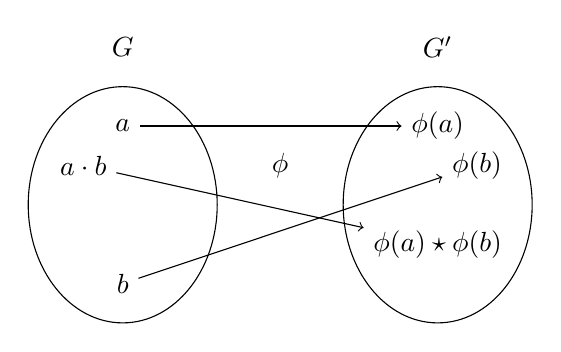
\begin{tikzpicture}
    \draw (-2,1.5) ellipse (1.2 and 1.5);
    \draw (2,1.5) ellipse (1.2 and 1.5);
    \node (v3) at (-2.5,2) {$a \cdot b$};
    \node (v1) at (-2,2.5) {$a$};
    \node (v5) at (-2,0.5) {$b$};
    \node (v2) at (2,2.5) {$\phi(a)$};
    \node (v4) at (2,1) {$\phi(a) \star \phi(b)$};
    \node (v6) at (2.5,2) {$\phi(b)$};
    \draw[->] (v1) edge (v2);
    \draw[->] (v3) edge (v4);
    \draw[->] (v5) edge (v6);
    \node at (-2,3.5) {$G$};
    \node at (2,3.5) {$G'$};
    \node at (0,2) {$\phi$};
  \end{tikzpicture}
  \caption{Isomorphismen lassen sich als Umbenennung der Gruppenelemente interpretieren.}
\end{figure}

Gibt es zwischen Gruppen $G$ und $G'$ einen Isomorphismus, so nennt man $G$ und $G'$ \emph{isomorph} und schreibt dies als $G \cong G'$.

Wir wollen uns die von verschiedenen Homomorphismen erzeugten Untergruppen genauer ansehen, da wir darüber Informationen über eine Gruppe erhalten können. Zwei Mengen sind hier von entscheidender Bedeutung:

\begin{definition}[Kern und Bild]
  Sei $\phi \colon G \rightarrow G'$ ein Gruppenhomomorphismus. Der \emph{Kern} von $\phi$ ist definiert als die Menge $\ker(\phi) = \left\{ g \in G \suchthat \phi(g)=e' \right\}$. Das \emph{Bild} von $\phi$ ist $\img(\phi) = \left\{ g' \in G' \suchthat \exists g \in G \text{ mit } \phi(g)=g'\right\}$.
\end{definition}

Der Kern und das Bild sollten selbst Untergruppen bilden, und das sind sie tatsächlich:

\begin{proposition}
  Ist $\phi \colon G \rightarrow G'$ ein Gruppenhomomorphismus, so gilt:
  \begin{enumerate}[label=\alph*)]
    \item $\ker(\phi) \leq G$
    \item $\img(\phi) \leq G'$
  \end{enumerate}
\end{proposition}

\begin{proof}
  \begin{enumerate}[label=\alph*)]
    \item Wir müssen zeigen, dass die Eigenschaften aus \reference{Definition}{def:algebra:untergruppe} gelten:
    \begin{enumerate}
      \item ist klar: $\phi(e)=e'$, also ist $e \in \ker(\phi)$.
      \item Angenommen, wir haben zwei Elemente $a,b \in \ker(\phi)$. Dann gilt die Gleichung $\phi(a \cdot b) = \phi(a) \star \phi(b) = e' \star e' = e'$, also ist auch $a \cdot b \in \ker(\phi)$.
      \item Sei $a \in \ker(\phi)$. Dann gilt $\phi(a^{-1}) = \phi(a)^{-1} = (e')^{-1} = e'$, somit ist auch $a^{-1} \in \ker(\phi)$.
    \end{enumerate}
    \item ist einfach, beziehungsweise analog zum ersten Teil.
  \end{enumerate}
\end{proof}

Auf der anderen Seite können wir auch Eigenschaften eines Homomorphismus aus dem Kern und Bild ablesen:

\begin{proposition}
  Ein Gruppenhomomorphismus $\phi \colon G \rightarrow G'$ ist genau dann injektiv, wenn $\ker(\phi) = \{e\}$.
\end{proposition}

\begin{proof}
  Wir zeigen die beiden Teile der Äquivalenz hintereinander.
  \begin{itemize}
    \item Wenn $\phi$ injektiv ist, so ist offensichtlich $\ker(\phi) = \{e\}$.
    \item Umgekehrt sei $\ker(\phi) = \{e\}$, und angenommen, es gäbe zwei Elemente $a,b \in G$ mit $a \neq b$ und $\phi(a) = \phi(b)$, also $\phi$ nicht injektiv. Dann gilt aber $a \cdot b^{-1} \neq e$ und $\phi(a\cdot b^{-1}) = \phi(a) \star \phi(b^{-1}) = \phi(a) \star \phi(b)^{-1} = \phi(a) \star \phi(a)^{-1} = e'$.
    Somit wäre $a \cdot b^{-1} \in \ker(\phi)$, was ein Widerspruch ist.
  \end{itemize}
\end{proof}

Schließlich wollen wir diesen Abschnitt mit einem interessanten Beispiel abschließen:

\begin{example}
  Wir wählen die zwei Gruppen $(\GL(n,\KK),\cdot)$ und $(\underbrace{\KK\setminus\{0\}}_{\eqqcolon \KK^\ast},\cdot)$, und betrachten die Abbildung
  \[\phi \colon \GL(n,\KK) \rightarrow \KK^\ast, \quad A \mapsto \det(A).\]

  Dann ist $\phi$ ein Gruppenhomomorphismus, weil nach Det.mult.satz gilt:\todowarning{Referenziere den DMS}
  \[\phi(A \cdot B) = \det(A \cdot B) = \det(A) \cdot \det(B) = \phi(A) \cdot \phi(B) \quad \forall A,B \in \GL(n,\KK).\]
\end{example}

\subsection{Links- und Rechtsnebenklassen}

\begin{definition}[Linksnebenklasse]
  Sei $G$ eine Gruppe und $H \leq G$. Eine Linksnebenklasse von $H$ in $G$ für ein $a \in G$ ist eine Teilmenge der Gestalt $a \cdot H = \left\{ a \cdot h \suchthat h \in H \right\}$.\todowarning{Bild}
\end{definition}

\begin{remark}
  Die Untergruppe $H$ selbst ist eine Linksnebenklasse, denn $H = 1 \cdot H$. Außerdem ist eine Linksnebenklasse von $H$ niemals leer, denn es gilt insbesondere $a \in aH$ mit $1 \in H$.
\end{remark}

\begin{lemma}[Linksnebenklassen]
  Für zwei Linksnebenklassen $aH$ und $bH$ von $H$ in $G$ sind äquivalent:
  \begin{enumerate}[label=\alph*)]
    \item $aH = bH$
    \item $aH \cap bH \neq \emptyset$
    \item $a \in bH$
    \item $b^{-1}a \in H$
  \end{enumerate}
\end{lemma}

\begin{proof}
  Wir werden den Ringschluss \emph{a)}$\Rightarrow$\emph{b)}$\Rightarrow$\emph{c)}$\Rightarrow$\emph{d)}$\Rightarrow$\emph{a)} zeigen.
  \begin{itemize}
    \item Die Implikation \emph{a)}$\Rightarrow$\emph{b)} ist klar.
    \item Für \emph{b)}$\Rightarrow$\emph{c)}, sei $c \in aH \cap bH$. Dann ist $c = a\cdot h_1$ und $c = b\cdot h_2$ für gewisse $h_1,h_2 \in H$ nach Definition der Linksnebenklassen. Also gilt $a\cdot h_1 = b\cdot h_2$, was allerdings impliziert, dass $a= b\cdot \underbrace{h_2\cdot h_1^{-1}}_{\in H} \in b \cdot H$ ist.
    \item Für \emph{c)}$\Rightarrow$\emph{d)} wissen wir, dass $a \in bH$ ist. Das heißt, $a = b\cdot h$ für ein gewisses $h \in H$. Aber dann ist wegen $b^{-1}\cdot a = h$ auch $b^{-1}\cdot a \in H$.
    \item Nun zur letzten Implikation \emph{d)}$\Rightarrow$\emph{a)}. Es gilt $b^{-1}\cdot a = h_0 \in H$, also $a=b\cdot h_0 \in bH$. Daher ist $a\cdot H = \left\{ a\cdot h \suchthat h \in H \right\} = \left\{ b\cdot h_0 \cdot h \suchthat h \in H \right\} \subseteq \left\{ b\cdot h' \suchthat h' \in H \right\} = b \cdot H$, kurz also $a\cdot H \subset b \cdot H$.
    Bleibt noch die umgekehrte Inklusion zu zeigen. Diese gilt jedoch nach dem gleichen Vorgehen, indem man benutzt, dass $(b^{-1}\cdot a)^{-1} = a^{-1} \cdot b \in H$ ist. Die Gleichheit gilt tatsächlich, denn offensichtlich ist $a^{-1}\cdot b \cdot b^{-1} \cdot a = 1$.
    Damit ist letztendlich $aH = bH$.
  \end{itemize}
\end{proof}

Das vorherige Lemma zeigt uns: Zwei Linksnebenklassen sind entweder gleich oder disjunkt.\todowarning{Bild} Jede Untergruppe $H \leq G$ induziert somit mittels Linksnebenklassen eine Partition von $G$.

\begin{theorem}[Mächtigkeit von Nebenklassen]

\end{theorem}

\begin{proof}

\end{proof}

\begin{remark}

\end{remark}}
